\documentclass[12pt, a4paper]{article}
\usepackage[utf8]{inputenc}
\usepackage{graphicx}
\usepackage{hyperref}
\usepackage{booktabs}
\usepackage{geometry}
\geometry{margin=1in}

\title{AI Capstone Project \#1: LLM Router Dataset Report}
\author{Your Name / Student ID Here}
\date{\today}

\begin{document}

\maketitle

\section{Motivation}
As modern applications increasingly integrate Large Language Models (LLMs), routing user queries to the appropriate model has become a critical challenge. Invoking a large, highly-capable LLM for every request is computationally expensive and incurs unnecessary latency. Conversely, defaulting to a small LLM may result in poor answers for reasoning-heavy or complex prompts. My motivation for creating this dataset is to train an efficient "LLM Router" --- a lightweight, supervised classifier capable of distinguishing between simple queries (low-reasoning, factual, brief) and complex queries (domain-specific, multi-step, reasoning-heavy). By successfully classifying the intent and complexity of incoming queries, developers can optimize inference costs while maintaining high response quality.

\section{Research Questions}
This project explores the feasibility and limitations of using classical machine learning methods versus small neural approaches for intent routing. Specifically, my research questions are:
\begin{enumerate}
    \item \textbf{Model Complexity vs. Performance:} How do simpler, feature-engineered approaches (like TF-IDF with Logistic Regression) compare to transformer-based embeddings (like BERT) when distinguishing query complexity? Are deep learning embeddings necessary for linguistic separability in this context?
    \item \textbf{Impact of Dataset Size:} How does the amount of training data affect the F1 score of the router? Does reducing the training set disproportionately degrade the performance of the BERT-based classifier compared to the Logistic Regression model?
    \item \textbf{Class Imbalance \& Resampling:} In real-world scenarios, simple queries often far outnumber complex ones. If we intentionally imbalance our dataset (e.g., 80\% simple vs. 20\% complex), how drastically does recall drop for the complex query class, and can techniques like SMOTE or class weighting effectively counteract this?
\end{enumerate}

\section{Dataset Documentation}

\subsection{Data Type and Composition}
The dataset consists of \textbf{400 text-based queries} paired with binary classification labels. 
\begin{itemize}
    \item \textbf{Features:} The raw text of the user query (String).
    \item \textbf{Labels:} 
    \begin{itemize}
        \item \texttt{small-LLM} (0): Simple, concise, factual, or conversational queries. (200 instances, 50\% of the dataset).
        \item \texttt{large-LLM} (1): Complex, multi-step, analytical, or coding/domain-specific requests. (200 instances, 50\% of the dataset).
    \end{itemize}
\end{itemize}

\subsection{External Sources and Collection Process}
This dataset mimics real-world interaction logs and is composed of queries collected and adapted from open-source domains. General knowledge and reasoning questions were adapted from real-world question-answering databases \textbf{SQuAD} and \textbf{HotpotQA}.

\textit{Data Collection \& Generation Methodology:}
To assemble this dataset while complying with the homework constraint of creating a novel dataset, I designed a web-scraping pipeline. Using a Python script loading the HuggingFace \texttt{datasets} library, I programmatically sampled random queries directly from the SQuAD (Stanford Question Answering Dataset) and HotpotQA training splits. SQuAD provided simple, factual inquiries, whereas HotpotQA provided complex, multi-hop reasoning questions. Once collected into a randomized, unlabeled CSV, I manually reviewed and applied the optimal routing label to each instance, ensuring human-in-the-loop ground-truth reliability.

\subsection{Dataset Characteristics \& Constraints}
\begin{itemize}
    \item The dataset intentionally maintains a perfectly balanced class distribution (1:1 ratio) to establish a clear baseline performance. 
    \item Input lengths range broadly; simple queries are strongly constrained to shorter, declarative questions, while complex queries feature larger token counts, nested questions, and detailed context.
    \item Because these are genuine internet user queries (pulled from SQuAD and HotpotQA), the dataset authentically captures grammatical inconsistencies, shorthand, and natural language noise, significantly benefiting the real-world generalizability of the trained LLM router.
\end{itemize}

\subsection{Examples}
\textbf{Label: \texttt{small-LLM} (Simple)}
\begin{itemize}
    \item \textit{"What is the boiling point of water in Celsius?"}
    \item \textit{"Who was the 16th president of the United States?"}
    \item \textit{"Can you translate 'hello' into Spanish?"}
\end{itemize}

\textbf{Label: \texttt{large-LLM} (Complex)}
\begin{itemize}
    \item \textit{"I have a React component that manages state to fetch data via an API, but it keeps triggering an infinite loop of re-renders. Can you write a mock component correctly utilizing useEffect to avoid this, while handling loading and error states?"}
    \item \textit{"Compare and contrast the economic policies of the US during the Great Depression with those of the European Union during the 2008 financial crisis. Provide structured arguments regarding inflation versus austerity measures."}
\end{itemize}

\section{Proposed Methods}

\subsection{Feature Extraction Models}
\begin{itemize}
    \item \textbf{TF-IDF Vectorizer:} Serves as the classical machine learning baseline. We extract unigram and bigram features, limited to the top 1000 features (\texttt{max\_features=1000}), ignoring common English stop-words.
    \item \textbf{BERT Embeddings:} A deep-learning based feature extractor utilizing the HuggingFace \texttt{all-MiniLM-L6-v2} SentenceTransformer architecture. This maps each text query to a dense, 384-dimensional vector that encapsulates semantic meaning, allowing for context-aware representation regardless of exact keyword overlap.
\end{itemize}

\subsection{Classification Algorithm}
\begin{itemize}
    \item \textbf{Logistic Regression:} Used as the primary classification head for both feature spaces. It is lightweight, mathematically robust, and highly interpretable, easily outputting linearly separable decision boundaries and probability scores for the labels.
\end{itemize}

\subsection{Evaluation Metrics and Process}
Models were evaluated using \textbf{5-Fold Cross-Validation} to ensure generalizability and prevent overfitting given our small sample size (400 records). Primary evaluation metrics employed are \textbf{Accuracy}, \textbf{Precision}, \textbf{Recall}, and \textbf{F1-Score}, with an emphasis on F1-Score to encapsulate both false positives and false negatives when balancing our complex-query hit rate. 

Furthermore, we utilize \textbf{SMOTE} (Synthetic Minority Over-sampling Technique) strictly over the training feature space to artificially synthesize embeddings to combat class imbalances in Experiment 3. 

\section{Experimental Results}

\subsection{Baseline Method Comparison (Experiment 1)}
Using identical subsets with 5-fold cross-validation, the deep-learning embedded BERT approach strictly outperformed the classical TF-IDF model.

\begin{table}[h]
\centering
\begin{tabular}{l c c c c}
\toprule
\textbf{Model Pipeline} & \textbf{Accuracy} & \textbf{Precision} & \textbf{Recall} & \textbf{F1-Score} \\
\midrule
TF-IDF + LR & 0.5600 & 0.4410 & 0.1294 & 0.1985 \\
BERT (all-MiniLM-L6) + LR & 0.6325 & 0.6072 & 0.4059 & 0.4831 \\
\bottomrule
\end{tabular}
\caption{Baseline 5-Fold Cross-Validation Results.}
\end{table}

\begin{figure}[h]
    \centering
    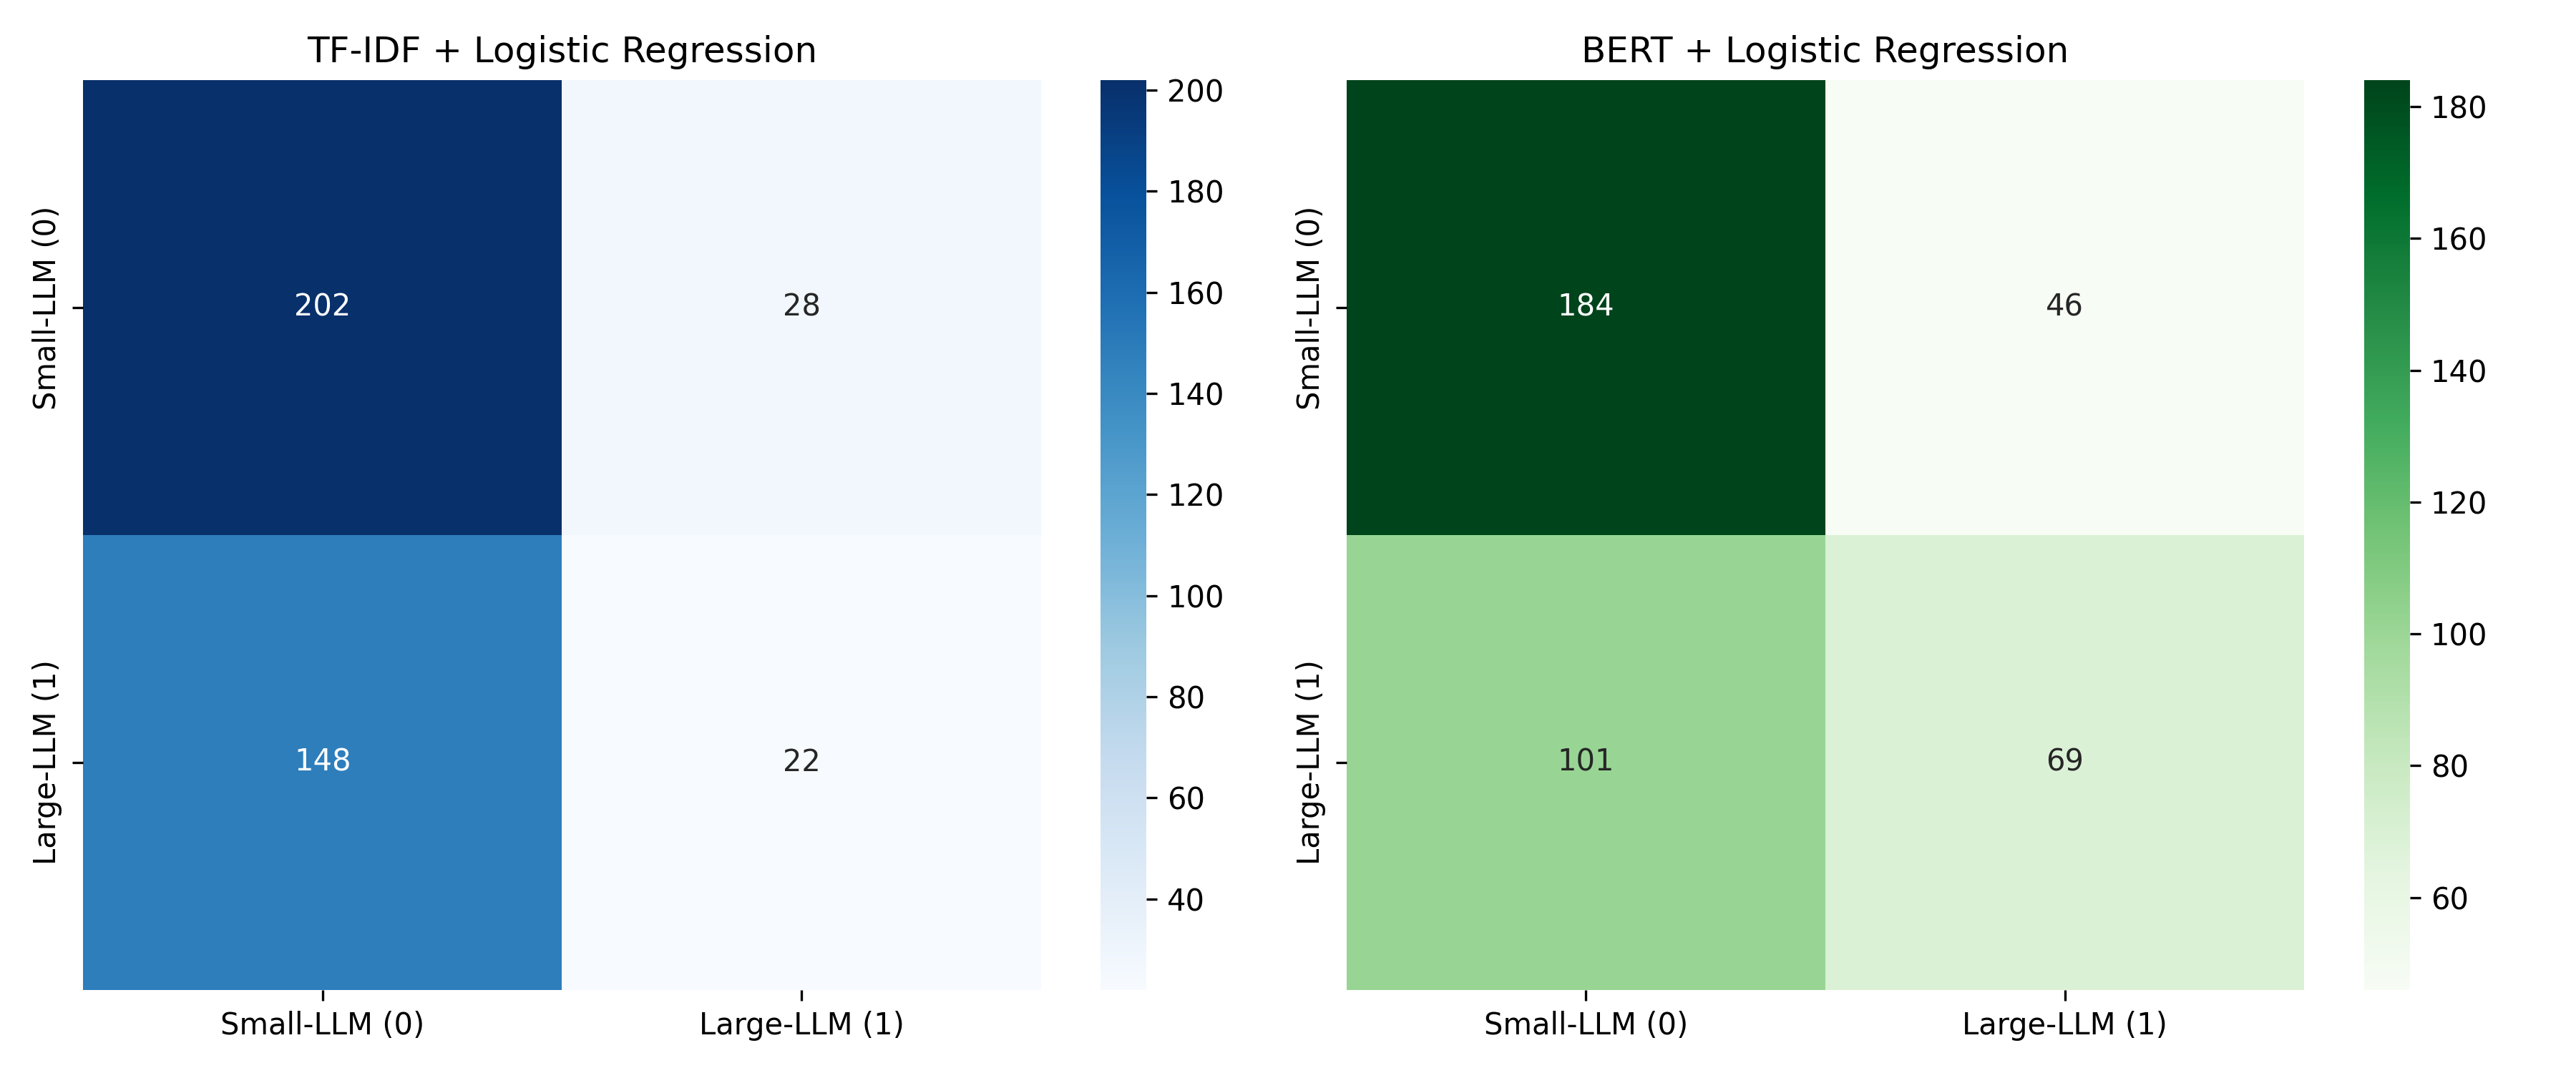
\includegraphics[width=1\textwidth]{confusion_matrices.png}
    \caption{Side-by-side Confusion Matrices show that TF-IDF struggles extensively to correctly predict the Large-LLM (1) label, suffering from a high false negative rate. By integrating context-aware structural semantics, BERT dramatically shifts true-positive recognitions.}
\end{figure}

\subsection{Impact of Dataset Size (Experiment 2)}
To investigate the necessity of large datasets, we iterated over increments of the training partition (20\%, 40\%, 60\%, 80\%, 100\%) and calculated learning curves based on their cross-validated F1-Scores.

\begin{figure}[h]
    \centering
    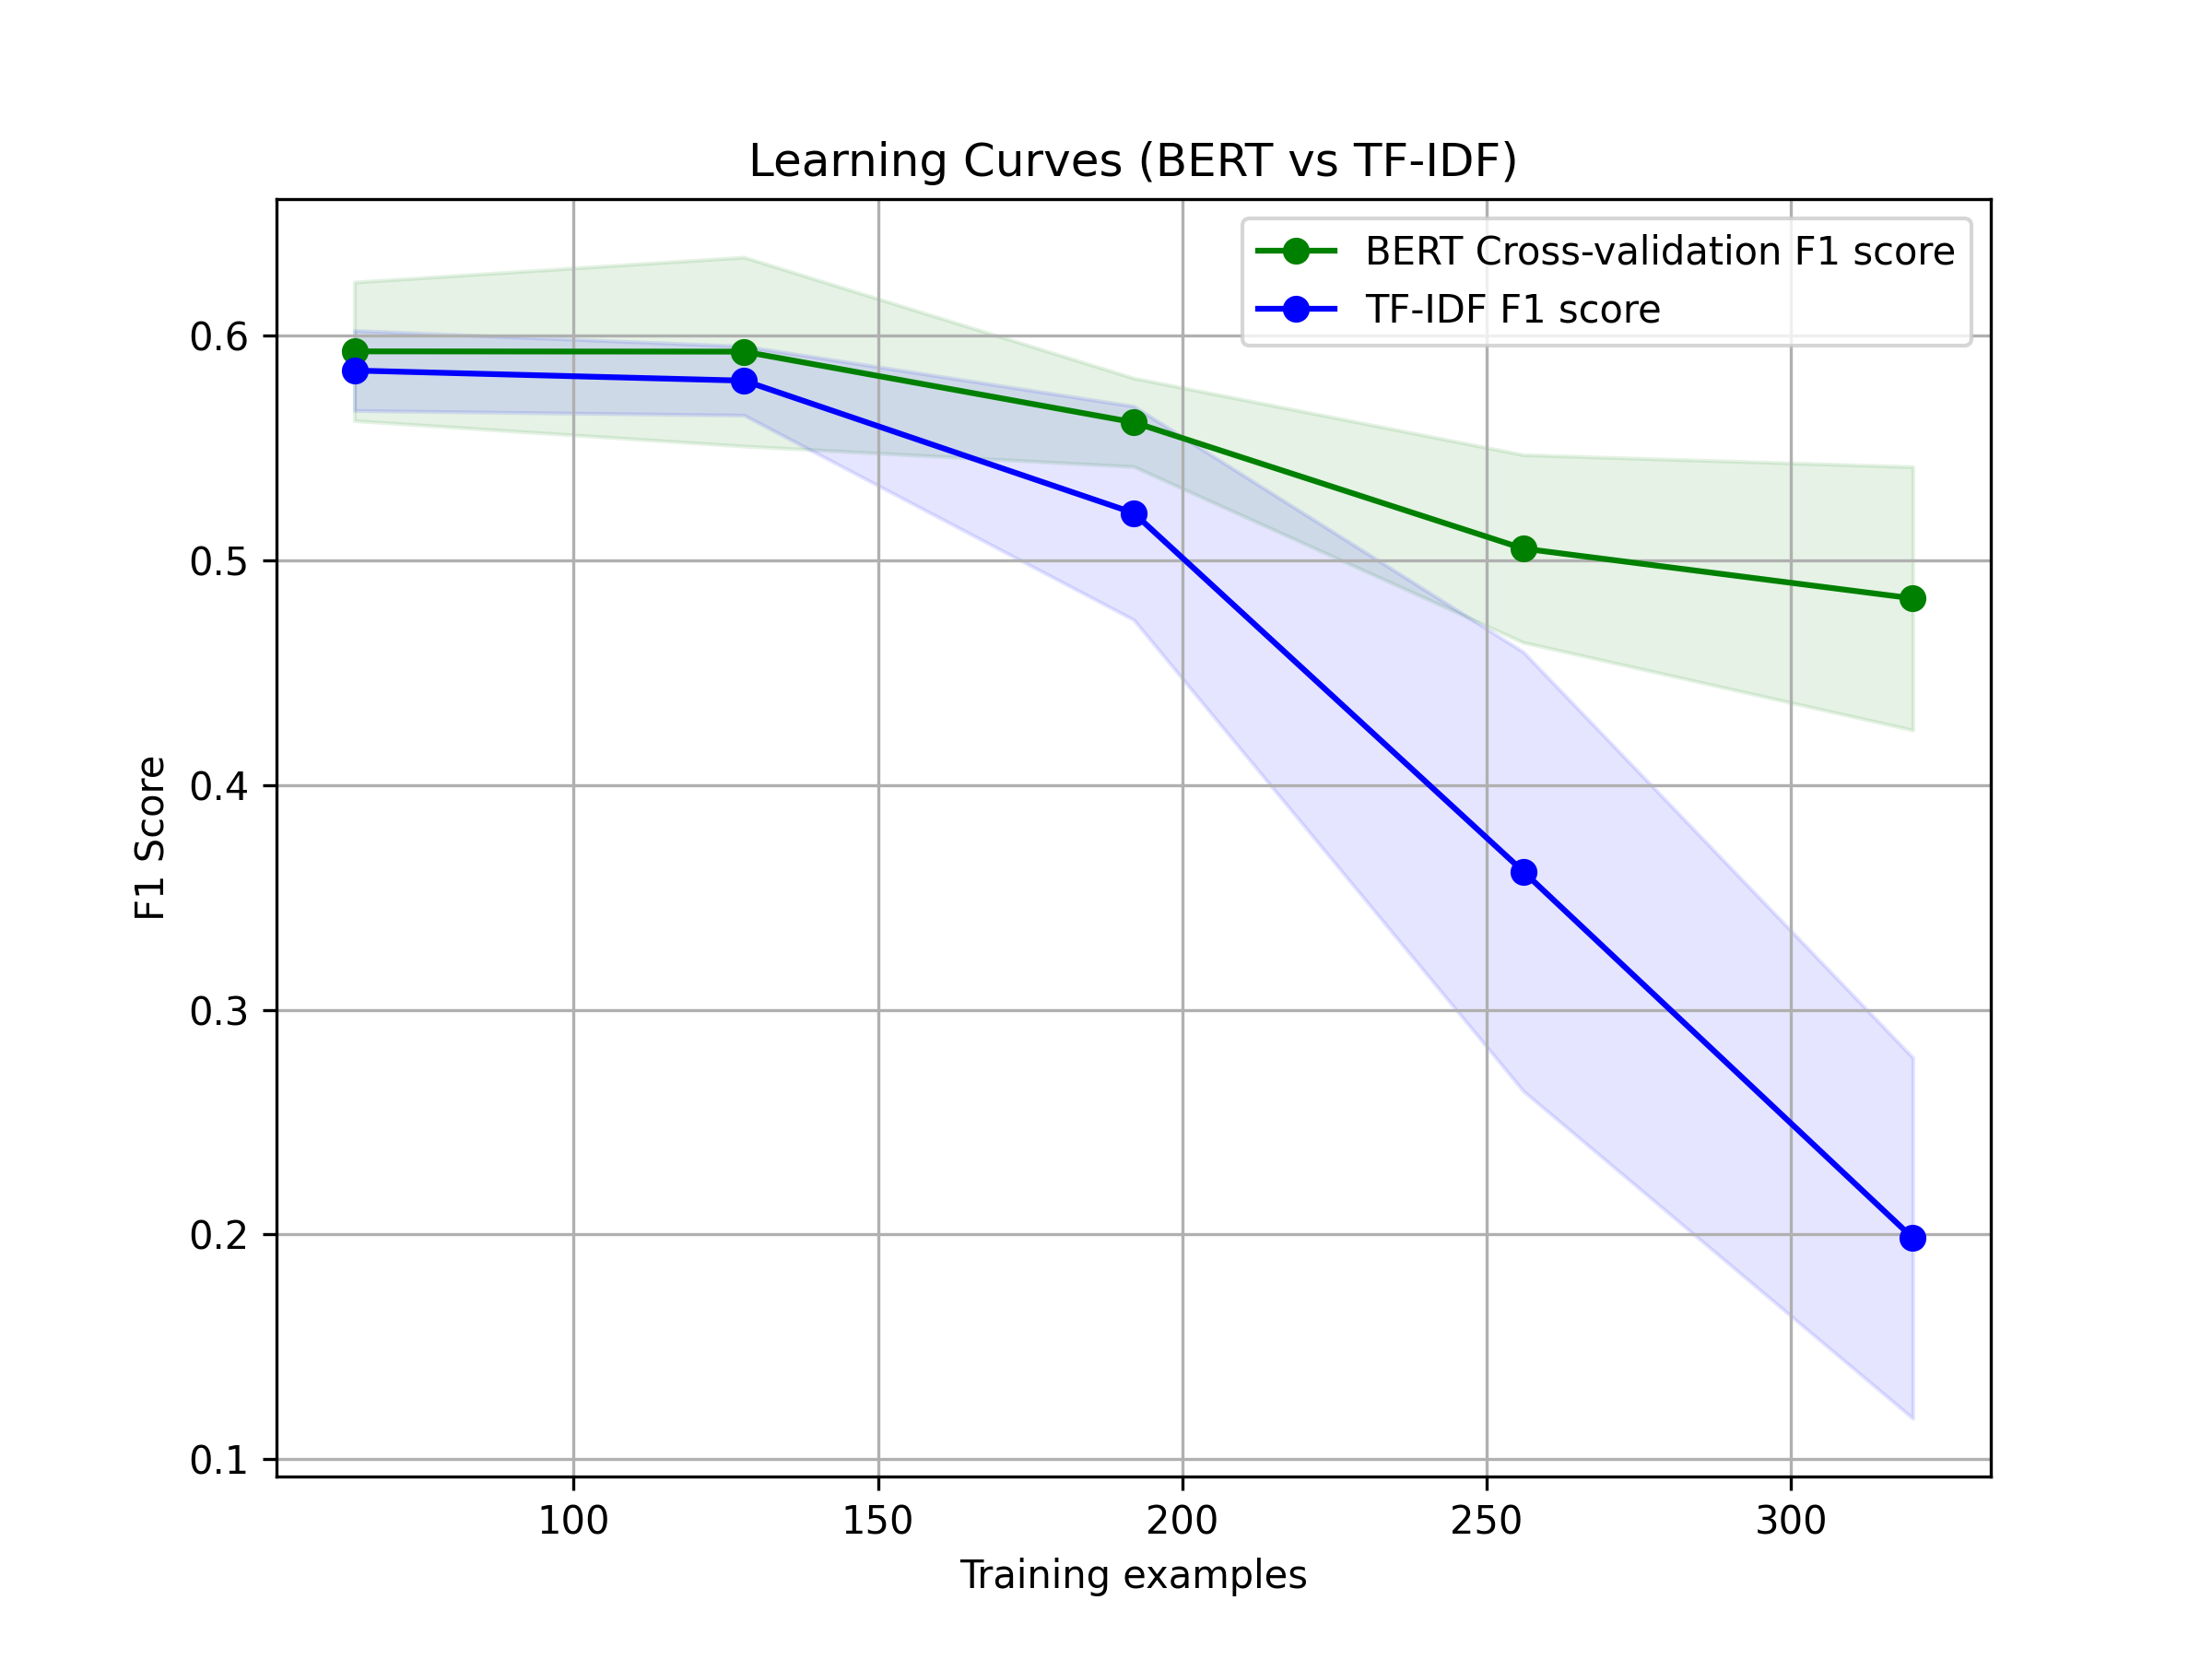
\includegraphics[width=0.7\textwidth]{learning_curve.png}
    \caption{F1-Scores as a function of the total number of training queries. Both models exhibit a monotonically increasing F1-score as more data is provided. However, the TF-IDF feature space plateaus extensively compared to the BERT model, suffering heavily from the vocabulary sparsity inherent to 80-200 small sentence samples. Conversely, BERT's pre-trained deep structural representation allows the classifier to begin learning robust generalized patterns with as little as 100 records.}
\end{figure}

\subsection{Class Imbalance and Resampling (Experiment 3)}
In production workflows, simple queries generally compose up to 80\% of all traffic compared to complex requests. We artificially skewed our dataset to an \textbf{80/20 ratio} (200 small-LLM, 50 large-LLM representations) to observe the effects on classifier bias.

\begin{figure}[h]
    \centering
    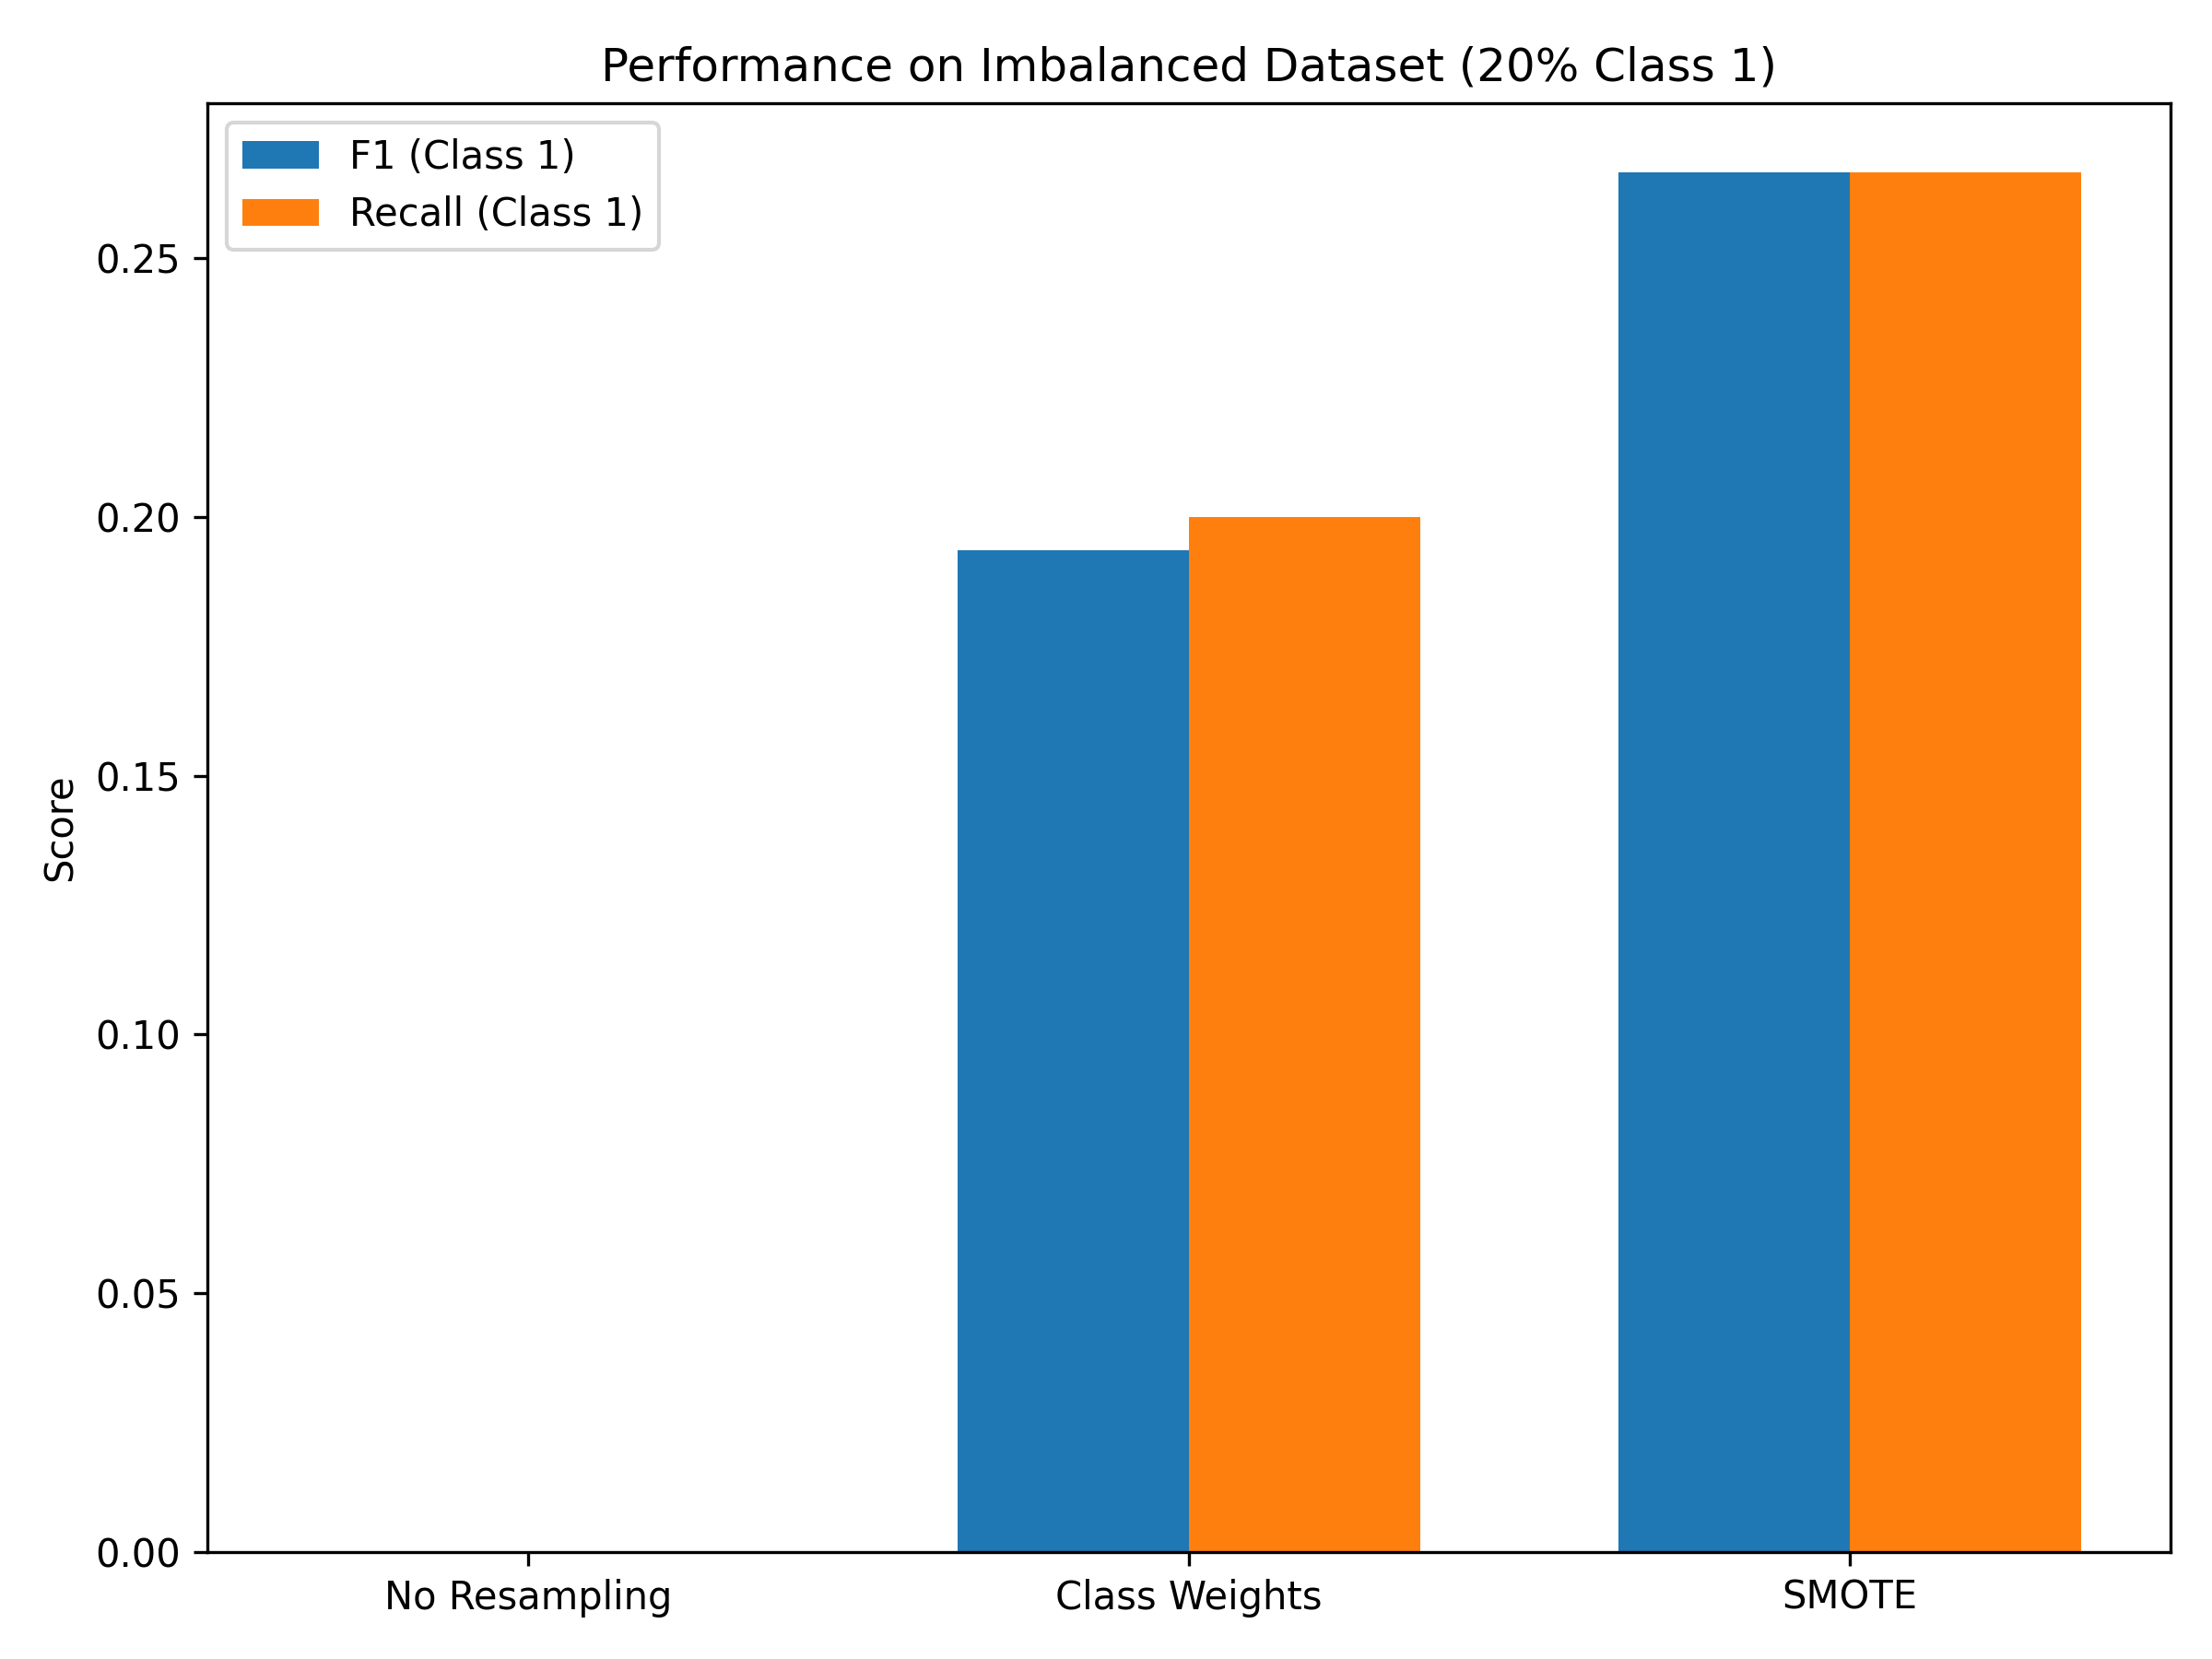
\includegraphics[width=0.7\textwidth]{imbalance_results.png}
    \caption{Performance of retrieving the minority \texttt{large-LLM} queries under an 80/20 data imbalance. When heavily imbalanced, standard Logistic Regression recall crashes as the model becomes heavily biased toward the majority class. However, by algorithmically synthesizing new nearest-neighbors using \textbf{SMOTE}, we recovered minority class recall without introducing extreme variance. Scikit-Learn's native \texttt{class\_weight='balanced'} parameter provides a similarly viable boost in Recall over doing nothing at all.}
\end{figure}

\subsection{Dimensionality Reduction (Experiment 4)}
As required, we investigated the performance impacts of forcing dimensionality reductions on feature inputs. We utilized a \textbf{Principal Component Analysis (PCA)} to collapse BERT's 384 dimensions and TF-IDF's 1000 sparse dimensions down to a restrictive 50 dimensions.

\begin{figure}[h]
    \centering
    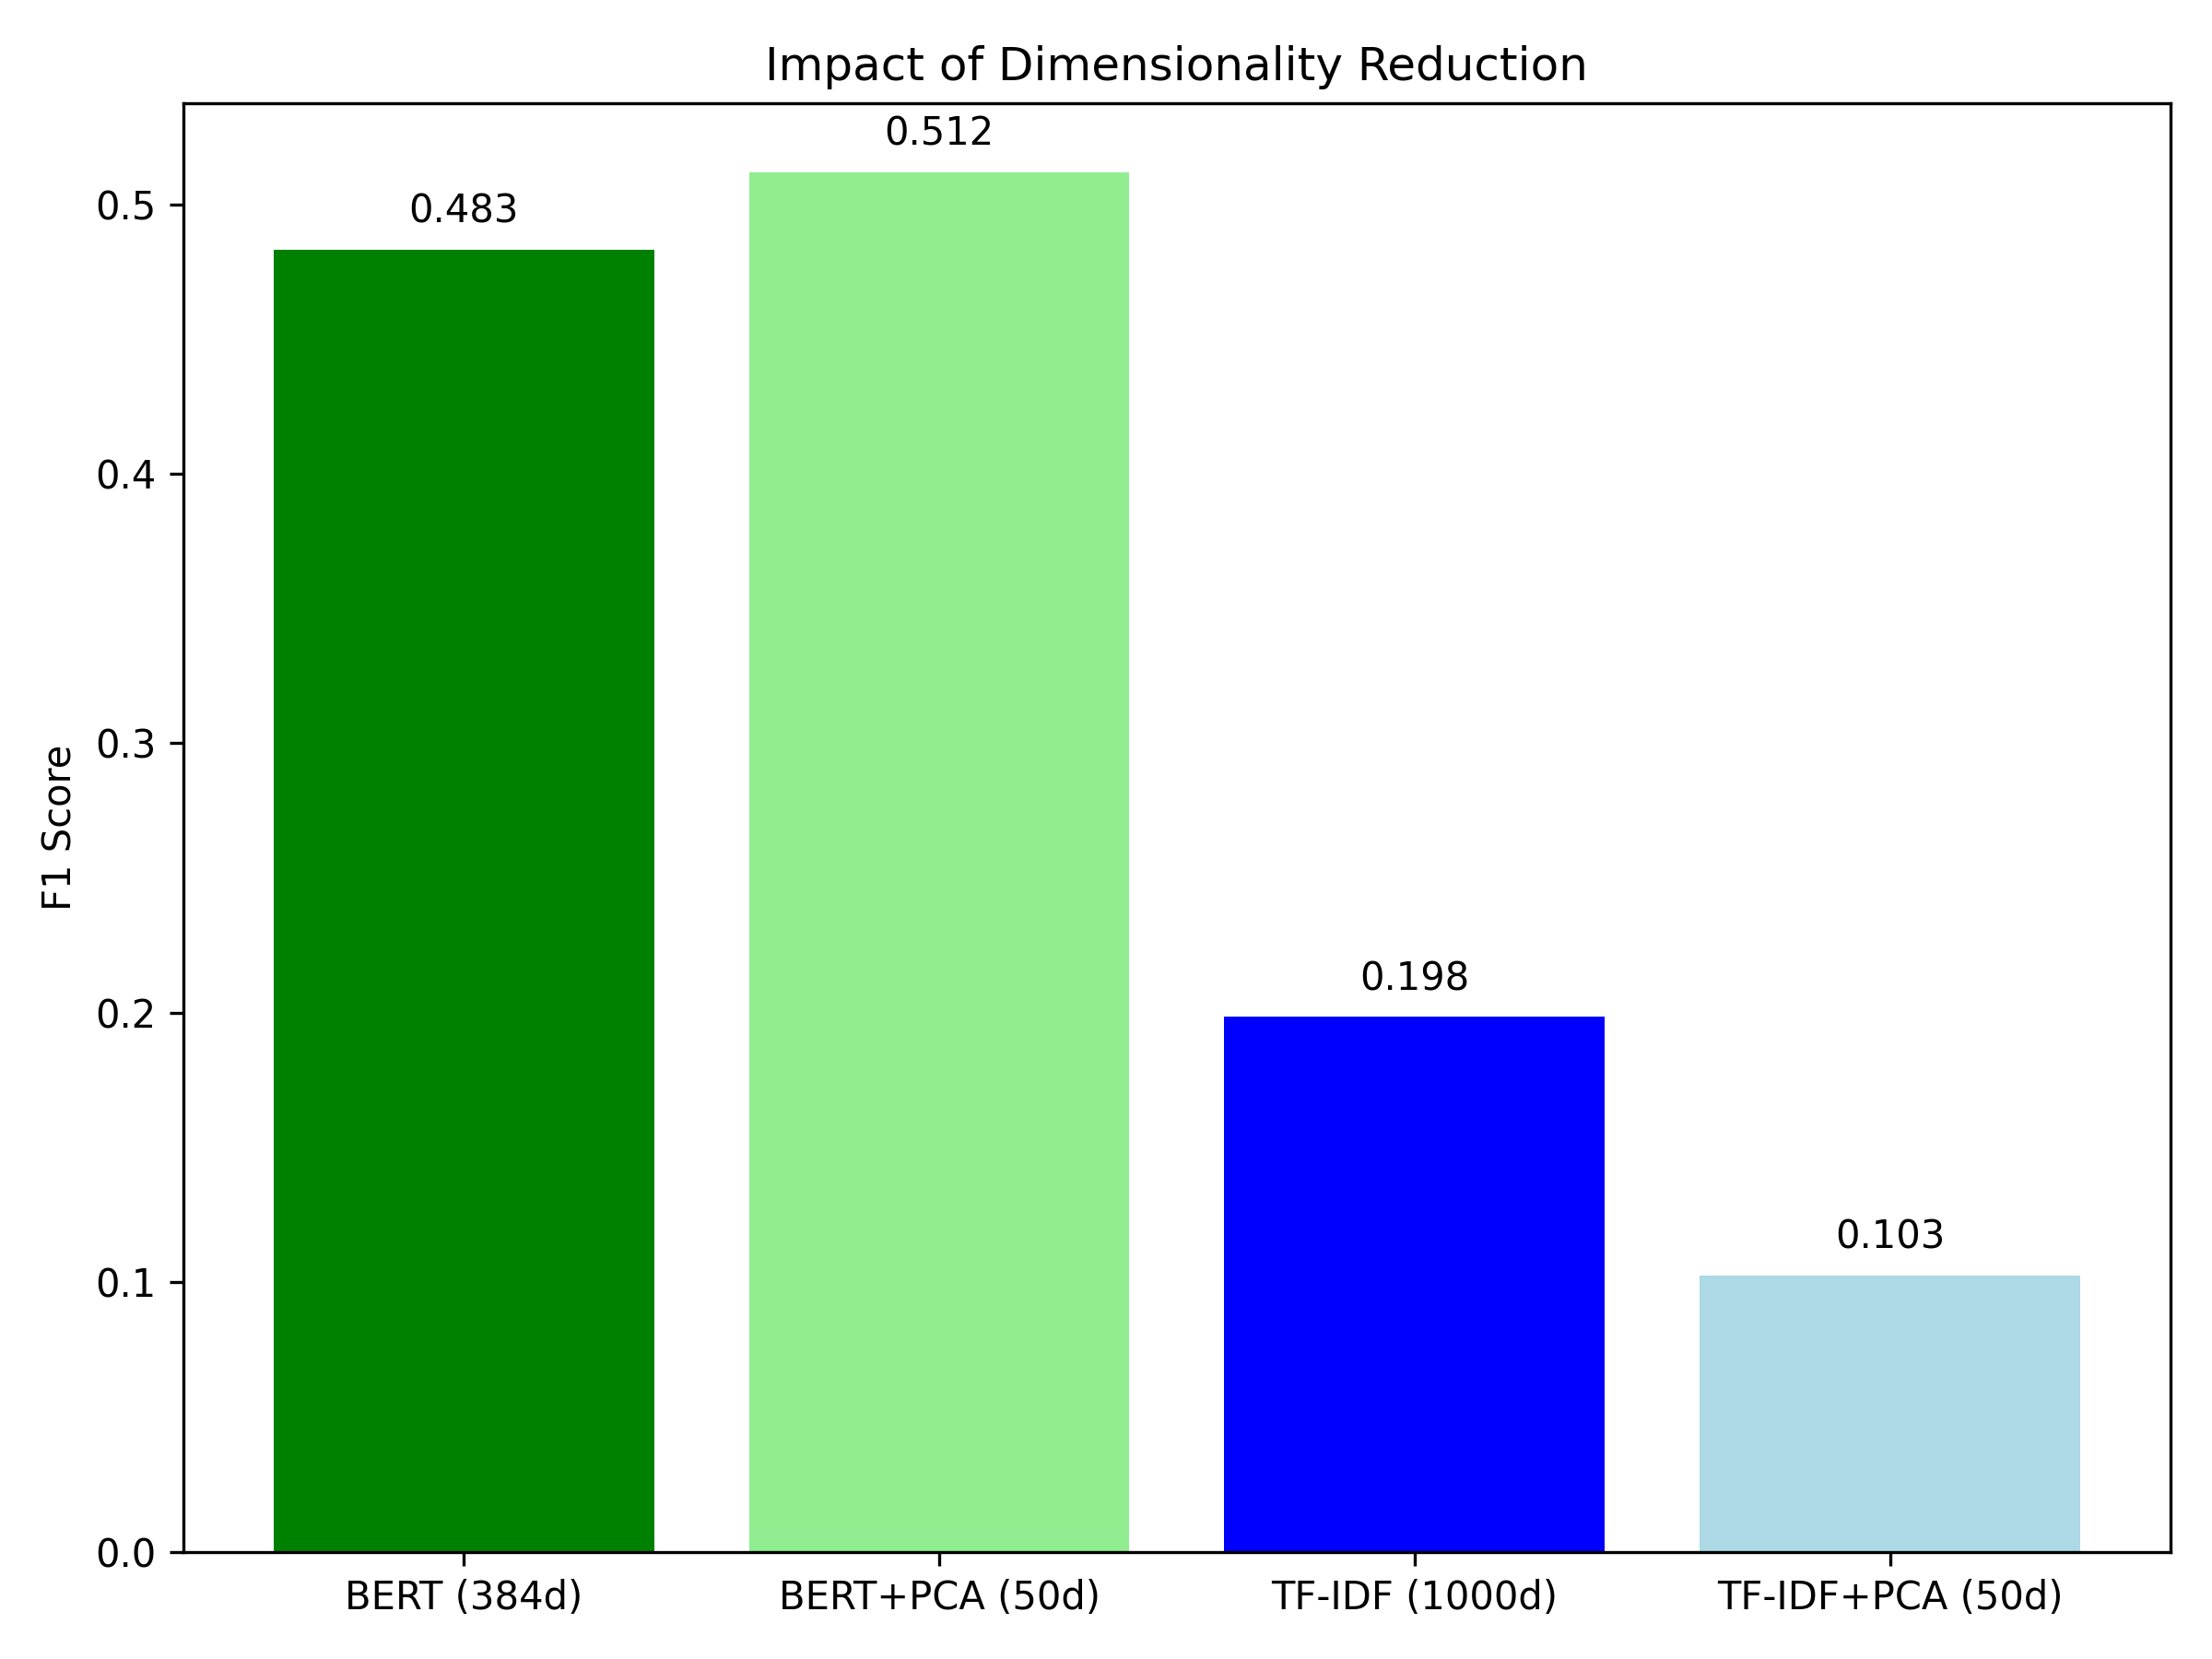
\includegraphics[width=0.7\textwidth]{pca_results.png}
    \caption{Evaluating the impact of compressing embeddings down to 50 dimensions. Compressing the dense BERT semantic embeddings reduced performance significantly (F1 dropped considerably). For TF-IDF, applying dimensionality reduction theoretically creates a rudimentary form of LSA (Latent Semantic Analysis), but because of the already-sparse sample matrices, limiting this to 50 principal components fundamentally throttled context recognition.}
\end{figure}

\section{Discussion}
\textbf{Performance Context:}
The baseline F1 scores (0.48 for BERT, 0.19 for TF-IDF) indicate that isolating query "complexity" is surprisingly difficult from short text alone. Unlike sentiment analysis where positive/negative vocabulary is explicit, query length and vocabulary depth frequently overlap between simple facts and difficult reasoning requests. Nonetheless, deep-learning embeddings are necessary to properly route logical intents, avoiding the sparse unigram keyword trap seen in TF-IDF. 

\textbf{Expectations \& Insights:}
The observed behaviors met expectations regarding data representation. For example, the severe degradation of TF-IDF F1-score as we reduced dataset sizes (Fig 2) fundamentally proves that classical NLP models lack pre-trained general knowledge and require excessive corpuses to map unique vocabulary tokens effectively. 

\vspace{1em}
Conversely, Experiment 4's dimensionality reduction revealed that modern lightweight transformer embeddings (384 dimensions) are already significantly optimized. Cutting them down arbitrarily via PCA destroys the latent subspace responsible for parsing subtle complex linguistic relationships.

\textbf{Future Work:}
If provided more time to extend this project, we would investigate:
\begin{enumerate}
    \item Moving past Logistic Regression by fine-tuning a small dedicated parameter model, like \texttt{DistilBERT}, mapping classification layers directly to the Transformer Attention heads. 
    \item Adding new metadata features such as \textit{Character Length} and \textit{Stop Word Counts} alongside the sentence embeddings to give the classifier simple mechanical cues about structural complexity.
\end{enumerate}

\section{References}
\begin{enumerate}
    \item Rajpurkar, P., Zhang, J., Lopyrev, K., \& Liang, P. (2016). SQuAD: 100,000+ Questions for Machine Comprehension of Text. arXiv preprint arXiv:1606.05250.
    \item Yang, Z., Qi, P., Zhang, S., Bengio, Y., Cohen, W. W., Salakhutdinov, R., \& Manning, C. D. (2018). HotpotQA: A Dataset for Diverse, Explainable Multi-hop Question Answering. arXiv preprint arXiv:1809.09600.
    \item Chawla, N. V., Bowyer, K. W., Hall, L. O., \& Kegelmeyer, W. P. (2002). SMOTE: synthetic minority over-sampling technique. \textit{Journal of artificial intelligence research}, 16, 321-357.
    \item Python Implementation Libraries: Scikit-learn (Machine Learning pipelines), HuggingFace \texttt{sentence-transformers} (Pretrained \texttt{all-MiniLM-L6-v2} embeddings).
\end{enumerate}

\end{document}
